\chapter{Simulation et Réalisation}
\section{Conception du logiciel}
\subsection{Description détaillée de la conception du logiciel}
\subsubsection{Architecture logicielle}
Ce système (SRI) est un système orienté WEB utilisant l'architecture MVC ou Modèle Vue Contrôleur. C'est un motif d'architecture logicielle destiné aux interfaces graphiques, lancé en 1978 et très populaire pour les applications web \citep{mvcwiki}.

Cet architecture est illustré dans la Figure~\ref{fig:mvc}

\begin{figure}[htbp]
    \begin{center}
        \fbox{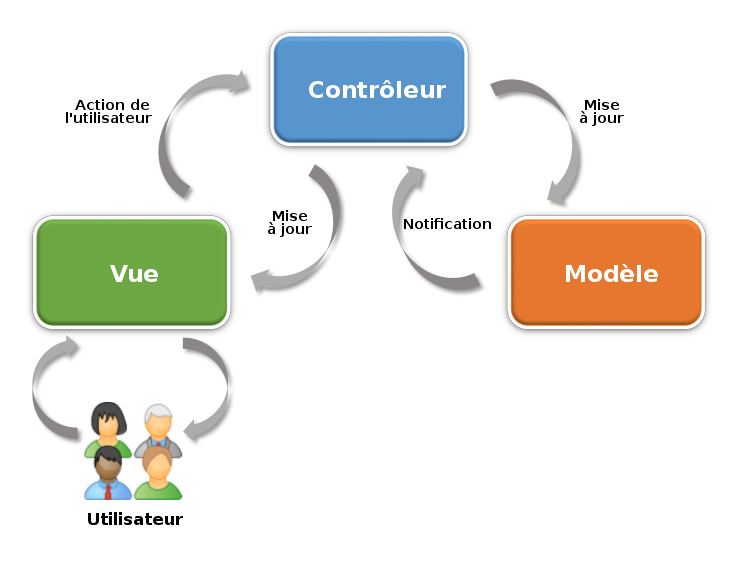
\includegraphics[width=13cm, angle=0]{Figures/Realisation/mvc.png}}
    \end{center}
    \caption{Architecture MVC \citep{mvcwiki}}\label{fig:mvc}
\end{figure}

\subsubsubsection*{Le Modèle (Model)}
Le Modèle contient les données a afficher a l'utilisateur. En d'autre terme, c'est la représentation de la base de données. Dans le cadre de ce système, l'index inversé, les documents ainsi que les catégorie des documents sont représenté par un modèle chacun.

\subsubsubsection*{La Vue (View)}
Elle contient la représentation graphique, tel que les formulaires, les listes, les tables, etc. Elle est généralement écrite en langage HTML pour une application WEB\@. Elle représente la formulaire de recherche, ainsi que les différents filtres de recherche par l'utilisateur, et aussi les parties concernant l'authentification et d'autres.

\subsubsubsection*{Le Contrôleur (Controller)}
Il contient la logique concernant les actions effectuées par l'utilisateur. En d'autre terme, il est le chef d'orchestre du système, traite les informations provenant de l'utilisateur et les persister dans la base de données et de récupérer des données et de les afficher a l'utilisateur. Dans ce système, il est responsable de tous traitement de documents, authentification, et d'autres traitements comme le téléchargement et protection des documents.

Il est utilisé par de nombreux frameworks pour applications web tels que ASP.NET MVC, Spring, Laravel, Django et d'autres.

\subsubsection{Choix de conception clés}
Pour ce système, on distingue deux type de conception tel que la \emph{conception de la base de données} et la \emph{conception de l'interface utilisateur}. Pour la base de données, deux approche sont possible tel que \emph{MERISE} et \emph{UML}. L'une de grande différence entre les deux ce que MERISE traite les données et les traitements séparément tandis que UML non.

\subsubsubsection*{MERISE}
Merise\footnote{\url{https://www.base-de-donnees.com/merise/}} est une méthode informatique dédiée à la modélisation qui analyse la structure à informatiser en terme de systèmes. Le gros avantage de cette méthode est qu’elle permet de cadrer le projet informatique et de \emph{discuter} en se comprenant entre utilisateurs et informaticiens.

Créée dans les années 70 sur commande de l’État français et destinée aux gros projets informatiques de l’époque, la méthode a perduré jusqu’à aujourd’hui. Son utilisation très répandue en Europe constitue un socle difficilement contournable lorsque l’on s’attache à la création de bases de données.

Merise est en fait un outil analytique qui facilite la création de base de données et de projets informatique. Le principal auteur de la méthode est Hubert \textbf{Tardieu} qui se basa sur les travaux autour du modèle relationnel de \textbf{Codd}.

Elle permet réellement de:
\begin{itemize}
    \item décrire le fonctionnement du système à informatiser tel que les \textbf{données} représenté par le \textbf{MCD} (Modèle Conceptuel de Données) qui détermine les relations et les dépendances entres les différents acteurs (utilisateur, administrateur, documents), et les \emph{traitements} représenté par le \textbf{MCT} (Modèle Conceptuel de Traitement) qui détermine comment les acteurs travaillent-ils ensemble.
    \item proposer une implémentation logique tel que \textbf{MLD} (Modèle Logique de Données), \textbf{MLT} (Modèle Logique de Traitement).
    \item Proposer une construction concrète et utilisable du point précédent tel que la \textbf{MPD} (Modèle Physique de Donnée).
\end{itemize}

\subsubsubsection*{UML}
Le Langage de Modélisation Unifié, de l'anglais \emph{Unified Modeling Language}\footnote{\url{http://uml.org/}}, est un langage de modélisation graphique à base de pictogrammes conçu comme une méthode normalisée de visualisation dans les domaines du développement logiciel et en conception orientée objet. L'UML est une synthèse de langages de modélisation objet antérieurs: Booch, OMT, OOSE.

Principalement issu des travaux de Grady Booch, James Rumbaugh et Ivar Jacobson, UML est à présent un standard adopté par l'Object Management Group. UML 1.0 a été normalisé en janvier 1997; UML 2.0 a été adopté par l'OMG en juillet 2005.

UML propose différentes diagrammes, et principalement catégorisé en trois catégories:

\begin{enumerate}
    \item \textbf{Structure}: Où on trouve
    \begin{itemize}
        \item \emph{Diagramme de classes}: Il montre la structure statique d'un système en mettant l'accent sur les classes du système, leurs attributs, leurs opérations et les relations entre les classes.
        \item \emph{Diagramme d'objets}: Il illustre des exemples spécifiques d'objets et de relations entre ces objets, montrant une instance particulière d'un diagramme de classes à un moment donné.
        \item \emph{Diagramme de composants}: Il met l'accent sur les composants d'un système logiciel et leurs dépendances, en montrant la structure des composants et la manière dont ils interagissent au niveau de l'architecture.
        \item \emph{Diagramme de paquetages}: Il organise les éléments d'un modèle en groupes, montrant comment ces éléments sont regroupés en paquets et les relations entre les paquets.
    \end{itemize}
    \item Comportement
    \begin{itemize}
        \item \emph{Diagramme de cas d'utilisation} Il décrit les interactions entre les utilisateurs et un système donné, mettant l'accent sur les fonctionnalités offertes par le système du point de vue de l'utilisateur.
        \item \emph{Diagramme de séquence} Il montre l'interaction entre les objets, en mettant l'accent sur la séquence temporelle des messages échangés entre les objets lors de l'exécution d'un scénario particulier.
        \item \emph{Diagramme d'activités} Il représente le flux de contrôle d'une activité ou d'un processus, mettant l'accent sur les actions et les décisions qui composent le processus.
        \item \emph{Diagramme d'états-transitions} Il modélise les transitions d'états pour un objet ou une entité donnée, montrant comment l'objet réagit aux événements au fil du temps.
    \end{itemize}
    \item \textbf{Déploiement}
    \begin{itemize}
        \item \emph{Diagramme de déploiement} Il montre la configuration matérielle d'un système et la manière dont les composants logiciels sont déployés sur cette configuration matérielle.
    \end{itemize}
\end{enumerate}

Ces différentes catégories de diagrammes UML offrent des moyens visuels efficaces pour modéliser les différents aspects d'un système logiciel, ce qui facilite la compréhension et la communication entre les différentes parties prenantes impliquées dans le processus de développement logiciel.

Dans le cadre de ce devoir, on utilisera l'approche UML, vu qu'on utilise une architecture MVC et une approche orienté objet (OOP), cette approche sera plus bénéfique.

Pour la conception de l'interface utilisateur, le langage de balisage \textbf{HTML5}, le feuille de style \textbf{CSS3} ainsi que le langage JavaScript est utilisé.

\subsubsubsection*{SGBD}
Un Système de Gestion de Base de Données est un logiciel système permettant aux utilisateurs et programmeurs de créer et de gérer des bases de données. Plus précisément, il permet a un ordinateur de stocker, récupérer,
ajouter, supprimer et modifier des données. Ce système est aujourd’hui utilisé dans presque tous les outils que nous utilisons \citep*{oracleDB}.

Le SGBD gère trois choses importantes: les \emph{données}, le \emph{moteur de base de données} qui permet d'accéder aux données, de les verrouiller et de les modifier, et le \emph{schéma de base de données}, qui définit la structure logique de la base de données. Ces trois éléments fondamentaux contribuent à assurer la concomitance, la sécurité, l'intégrité des données et l'uniformité des procédures administratives \citep*{oracleDB}.

\subsubsection{Les fonctionnalités de base}
Citons les fonctionnalités de base qui sont le plus importants pour ce système.
\begin{enumerate}
    \item \textbf{Indexer des documents}: capacité d'indexer des documents textuelles de différente format tel que PDF, WORD. Cette fonctionnalité inclus l'extraction automatique de titre, résumé, date de soutenance, ainsi de faire un traitement de langage naturel. Cette fonctionnalité se fait par un téléversement de fichier via un navigateur WEB\@.
    \item \textbf{Système d'authentification}: permet a l'utilisateur de s'authentifier ou se créer des comptes afin de déposer et télécharger des documents. Elle permet aussi aux administrateurs de valider des documents, les supprimer si nécessaire. Elle permet aussi de disposer d'un espace membre en tant qu'étudiant et en tant qu'enseignant, verrouiller des documents et de ne donner l'accès qu'a certains utilisateurs.
    \item \textbf{Recherche par mots clés}: cette fonctionnalité permet aux utilisateurs de faire des recherches en utilisant une zone de saisie par des mots clés afin de satisfaire ses besoins. Cette fonctionnalité inclus d'autres fonctionnalités tel que le \emph{système de filtre de recherche}: recherche par contenu, par titre ou par auteur; \emph{système de filtre d'organisation}: par année croissante ou décroissante, par université; \emph{traitement de la requête}: suppression des mots vides, correction des orthographes, pondération du terme de la requête. Elle se charge de faire l’appariement entre la requête de l'utilisateur et les documents dans la collection, et afficher ensuite les résultats par ordre de pertinence décroissante. L'utilisateur peut avoir une suggestion des mots clés lorsqu'il exprime son besoin d'information.
    \item \textbf{Page de résultat et visualisation de document}: permet d'afficher les résultats avec des paginations, ainsi que la possibilité de visualiser le résumé ou la partie du document. Il est aussi possible de visualiser un document en entier.
\end{enumerate}

\subsubsection{Quelques diagrammes}
Illustrons quelques diagrammes utilisant l'approche UML\@.

\subsubsubsection*{Diagramme de cas d'utilisation}
Le diagramme de cas d'utilisation illustrant les fonctionnalités du système est illustré dans la Figure~\ref{fig:dcu}.

\begin{figure}[htbp]
    \begin{center}
        \fbox{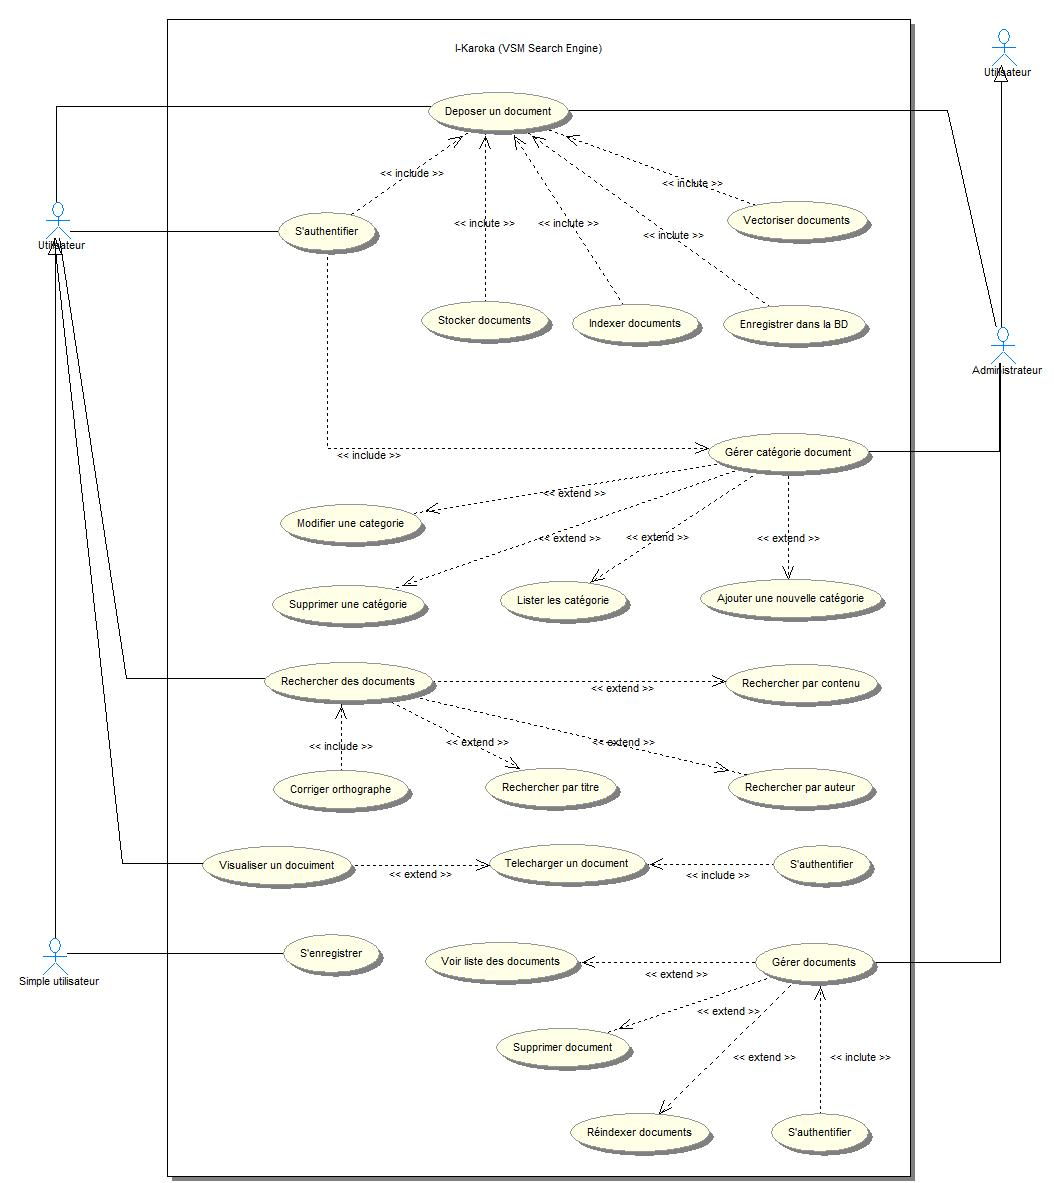
\includegraphics[width=13cm, angle=0]{Figures/Realisation/Diagrammes/Diagramme de cas d'utilisation.jpg}}
    \end{center}
    \caption{Diagramme de cas d'utilisation}\label{fig:dcu}
\end{figure}

\subsubsubsection*{Diagramme de classe}
Le diagramme de classe illustrant les entités ainsi que les relations entre eux, est illustré dans la Figure~\ref{fig:dc}.

\begin{figure}[htbp]
    \begin{center}
        \fbox{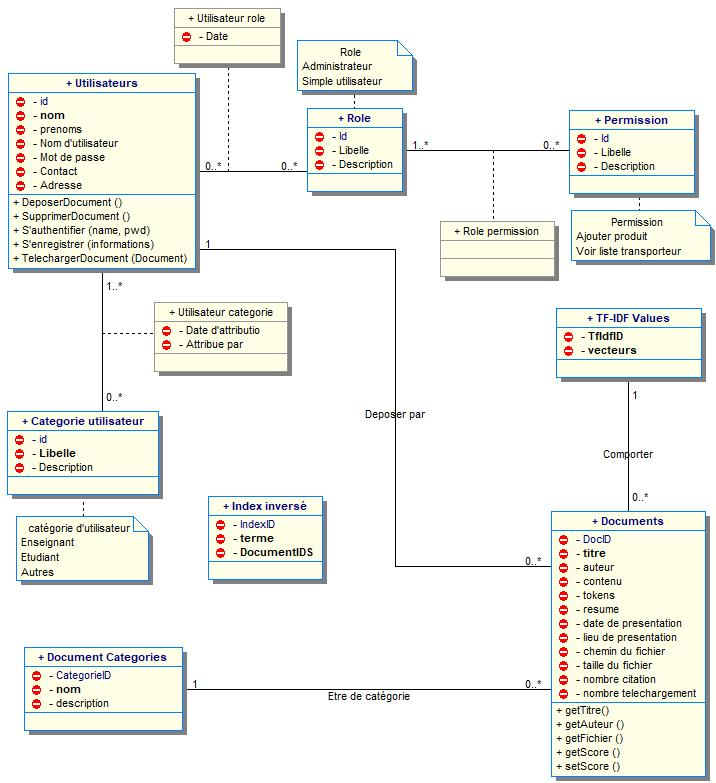
\includegraphics[width=13cm, angle=0]{Figures/Realisation/Diagrammes/Diagramme principale.jpg}}
    \end{center}
    \caption{Diagramme de classe}\label{fig:dc}
\end{figure}

\subsubsubsection*{Diagramme d'activités}
Le diagramme d'activités sont illustré dans la Figure~\ref{fig:search}, et dans la Figure~\ref{fig:upload}.
\begin{figure}[htbp]
    \begin{center}
        \fbox{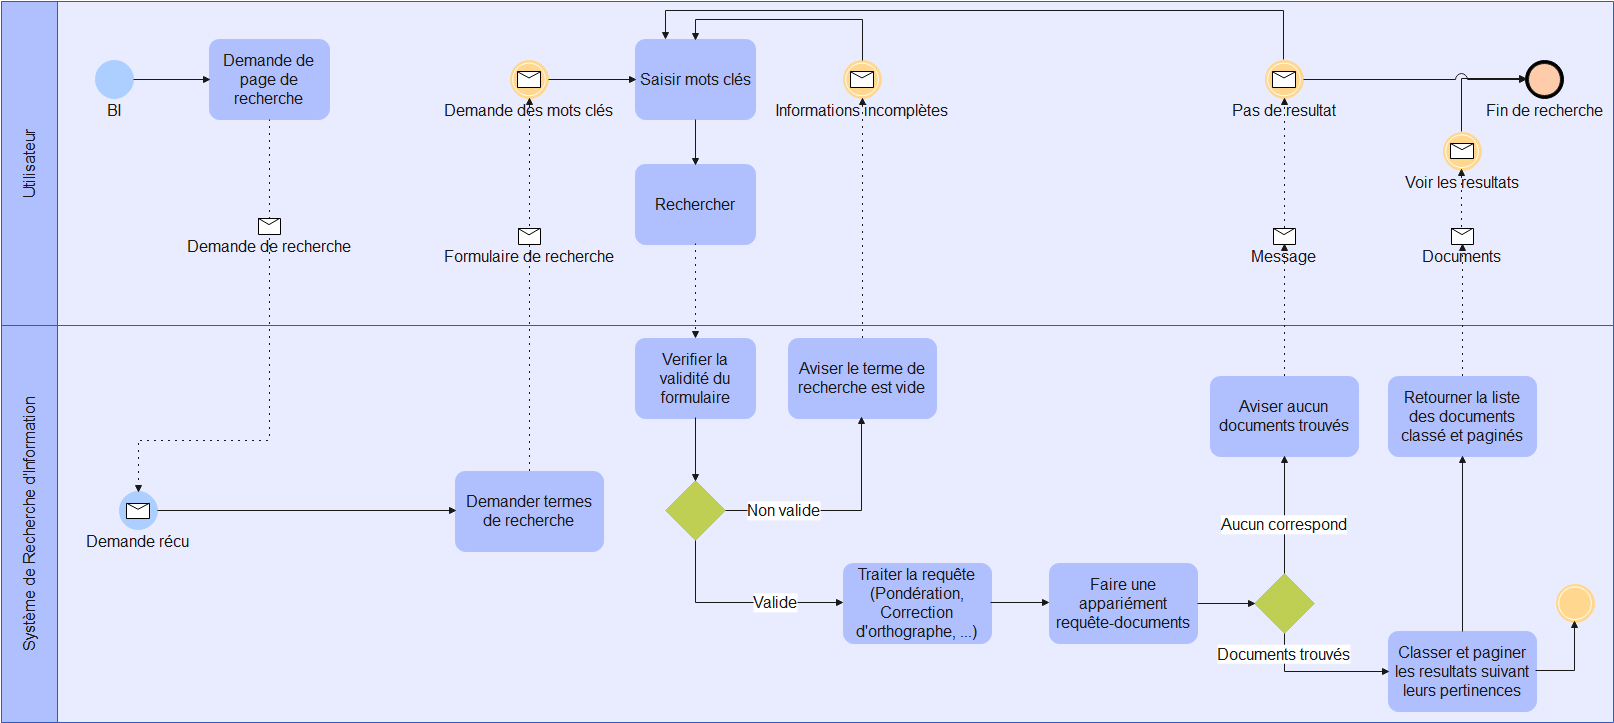
\includegraphics[width=13cm, angle=0]{Figures/Realisation/Diagrammes/Activites/Rechercher des documents.png}}
    \end{center}
    \caption{Rechercher des documents}\label{fig:search}
\end{figure}

\begin{figure}[htbp]
    \begin{center}
        \fbox{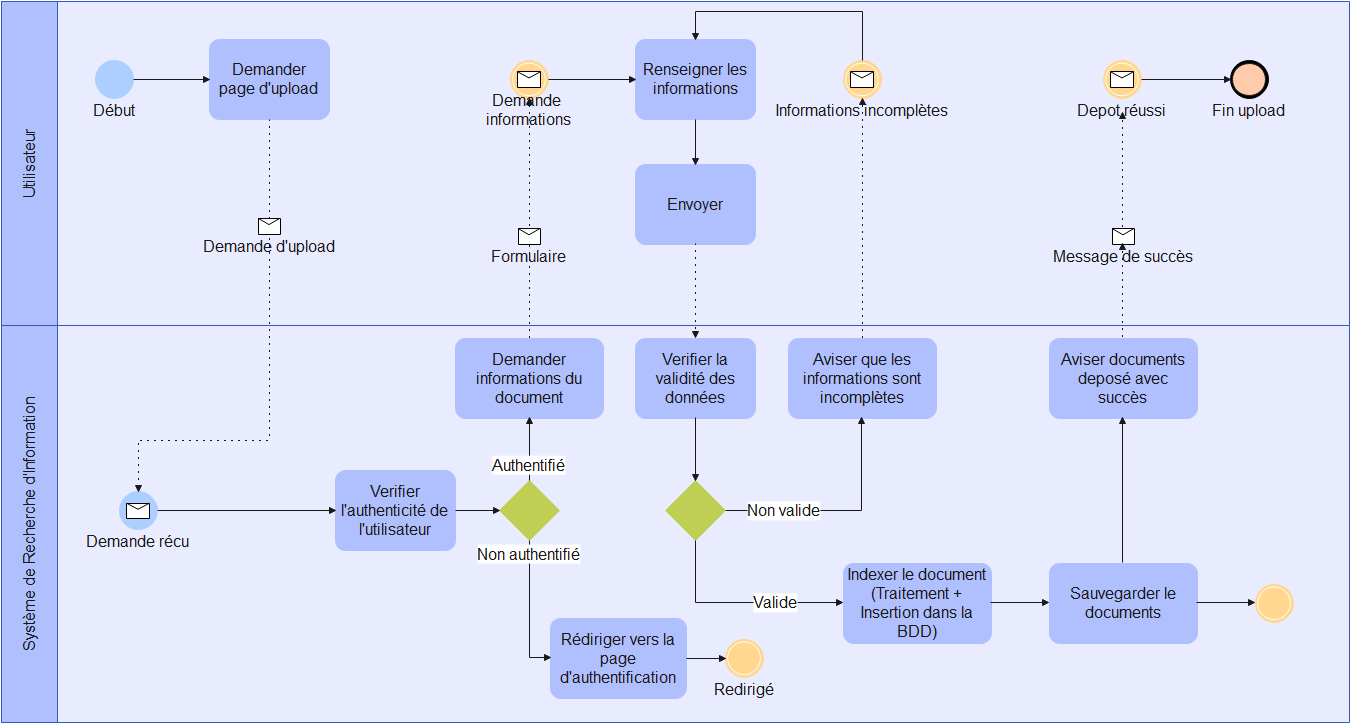
\includegraphics[width=13cm, angle=0]{Figures/Realisation/Diagrammes/Activites/Upload document.png}}
    \end{center}
    \caption{Déposer un document}\label{fig:upload}
\end{figure}

\subsection{Technologies et outils utilisés}
\subsubsection{Technologies}
Pour développer ce SRI, on a utilisé des technologies orientés vers l'intelligence artificiel implémenté dans un application web. On aura utilisé une base de données pour stocker les données tel que les documents, les informations de l'utilisateur, etc. Ci-dessous la liste des technologies utilisés pour la réalisation de ce système.

\begin{itemize}
    \item \textbf{Framework Django}\footnote{\url{https://www.djangoproject.com/}}: est un framework web développé en langage Python utilisant l'architecture MVT (Model-View-Template). A bien noter que dans Django, View est l’équivalent d'un Contrôleur et que Template est l’équivalent de Vue. Ce choix est dû au fait qu'il est facile d’intégré des librairies d'intelligence artificiel dans ce framework, ainsi que les fonctionnalités pré-conçus facilitera beaucoup le développement.
    \item \textbf{MySQL}\footnote{\url{https://www.mysql.com/fr/}}: pour stocker les données comme on a dit ci-dessus. Elle est gratuite et largement suffisant pour ce genre de système en terme de capacité de stockage et en terme de rapidité de récupération des données.
    \item \textbf{Spacy}\footnote{\url{https://spacy.io/}}: est un librairie python permettant de faire un traitement de langage naturel. Il utilise un modèle de \emph{machine learning} pré-entraîné pour différentes langages. Comme pour la langue française tel que le modèle \emph{\texttt{fr\_core\_web\_news\_sm}}, \emph{\texttt{fr\_core\_web\_news\_md}} et \emph{\texttt{fr\_core\_web\_news\_lg}}. Ce librairie permet de segmenter des textes en français, supprimer les mots vides, et récupérer la racine des mots, c'est ce librairie qui se charge de l'indexation dans ce SRI\@.
    \item \textbf{NLTK}\footnote{\url{https://www.nltk.org/}}: ou Natural Language Toolkit est aussi une librairie de traitement de langage naturel. Il permet aussi d'utiliser la base de connaissance tel que \emph{WordNet} pour trouver des synonymes des mots.
    \item \textbf{Numpy}\footnote{\url{https://numpy.org/}}: est un librairie open source pour les calculs scientifiques avec python. Il est rapide et performant pour une vectorisation et calcul matriciel de N dimension.
    \item \textbf{ScikitLearn}\footnote{\url{https://scikit-learn.org/}}: est une bibliothèque logicielle libre d'apprentissage automatique pour le langage de programmation Python. Elle propose divers algorithmes de classification, de régression et de regroupement, notamment des machines à vecteurs de support (SVM), des forêts aléatoires (Random Forest), du boosting de gradient (Gradient boosting), des k-moyennes et DBSCAN, et est conçue pour interagir avec les bibliothèques numériques et scientifiques Python, NumPy et SciPy.
    \item \textbf{PyMuPDF}\footnote{\url{https://pymupdf.readthedocs.io/en/latest/index.html}}: PyMuPDF est une bibliothèque Python très performant pour l'extraction de données, l'analyse, la conversion et la manipulation de documents PDF et d'autres documents. Dans le cadre de ce système, cette librairie se charge d'extraire les contenus des documents PDF\@.
    \item \textbf{Spellchecker library}\footnote{\url{https://pypi.org/project/pyspellchecker/}}: Pure Python Spell est utilisé pour corriger des fautes d'orthographes. Elle utilise l'algorithme de \emph{distance de Levenshtein} pour déterminer le vrai mot. Dans le cadre de ce système, cette librairie se charge de corriger la faute d'orthographe dans les mots clés de l'utilisateur qui composent son requête.
\end{itemize}

\subsubsection{Langage de programmation}
Diverses langages de programmation sont utilisés dans le cadre de ce système. Pour la programmation de base (Côté serveur), on a utilisé le langage de programmation \textbf{Python}\footnote{\url{https://www.python.org/}} par sa facilité d’interagir avec les librairies de Machine Learning (ML) et du Deep Learning (DL). Python est un langage open source, multi-plateforme, spécialisé dans le domaine de l'intelligence artificiel et de l'analyse de données.

Pour la partie interface utilisateur, le langage HTML, CSS et JavaScript sont utilisés. Et le langage SQL pour le langage de requête a la base de données.

\subsubsection{Outils}
Diverses outils sont utilisés dans le cadre de ce système:

\begin{itemize}
    \item \textbf{Environnement de Développement Intégré (IDE)}: on a utilisé \emph{Visual Studio Code}\footnote{\url{https://code.visualstudio.com/}}, qui est un outils crée par Microsoft, OpenSource, gratuit et propose des diverses extensions pour faciliter le développement (compréhension du langage python par exemple).
    \item \textbf{Gestion de version}: \emph{Git}\footnote{\url{https://git-scm.com/}} et \emph{Github}\footnote{\url{https://github.com/}} sont l'un de plus populaire pour mieux organiser les versions d'un système et propose système de travail en équipe.
    \item \textbf{Ordinateur utilisé}: ce système est realisé avec un ordinateur de processeur \textbf{Pentium G3200 @ 3300 Ghz}, avec \textbf{8GB de RAM}, et une \textbf{carte graphique Intel Graphic HD 4800} sous un système d'exploitation \textbf{KALI Linux 2022.3}.
    \item \textbf{Outil de test}: l'outil de test est intégré directement dans le framework Django.
\end{itemize}

\section{Développement du logiciel}
\subsection{Étapes du processus de développement}
\subsubsection{Planification}
L'identification des fonctionnalités se fait par l'analyse des moteurs de recherche existants pour déterminer les fonctionnalités intéressantes ainsi que de trouver les fonctionnalités manquantes et des lacunes. Une fois la liste des fonctionnalités nécessaires déterminés, l'identification des acteurs du système est mis en place. Une fois terminé, la modélisation de ces informations est faite en utilisant les diagrammes proposé par l'approche UML\@.

\subsubsection{Programmation}
D'abord, le système de sécurité est mis en place pour pouvoir déposer des documents, y compris la création de compte, authentification ainsi que la mise en place de certains contraintes pour les utilisateurs. Ensuite, la fonctionnalité d'indexation des documents, y compris la création des index inversés, et tous les traitements rattachés a l'étape d'indexation (normalisation, lemmatisation). Ainsi le développement de la partie recherche ou l'utilisateur peut récupérer la liste des documents qui répondent a son besoin, y compris la page de résultat. Et après la gestion des téléchargement des documents, gestion d’aperçu es documents. Enfin la fonctionnalité de gestion du système par l'administrateur comme suppression des documents, des utilisateurs, modification des droits d'accès.

Illustrons quelques algorithmes pour le fonctionnement de ce système.

\begin{algorithm}
    \caption{Téléversement de document}
    \begin{algorithmic}[1]
    \State \textbf{Données:} Requête HTTP
    \State \textbf{Résultat:} Redirection de l'utilisateur ou rendu du formulaire de téléchargement
    
    \State \textbf{Entrée:} request: HttpRequest
    \State \textbf{Sortie:} Redirection de l'utilisateur ou rendu du formulaire de téléchargement
    
    \State Assurez-vous que l'utilisateur est connecté
    
    \If{La méthode de la requête est 'POST'}
        \State Extraire le titre, l'auteur et la catégorie du document de la requête
        \State Vérifier l'existence du fichier et le sauvegarder s'il n'existe pas
        
        \State Extraire le contenu textuel et le résumé du document
        \State Diviser le contenu en jetons individuels \Comment{Indexation}
        \State Convertir les jetons en vecteurs numériques \Comment{Vectorisation}
        
        \State Sauvegarder le document dans la base de données
        \State Mettre à jour l'index inversé pour chaque terme
        \State Mettre à jour les vecteurs TF-IDF
        
        \State Rediriger l'utilisateur vers la page de téléchargement
    \Else
        \State Rendre le formulaire de téléchargement avec les catégories disponibles
    \EndIf
    \end{algorithmic}
\end{algorithm}

\begin{algorithm}
    \caption{Sauvegarder le Fichier Téléchargé}
    \begin{algorithmic}[1]
    \Function{handle\_uploaded\_file}{$f, dossier$}
        \State \textbf{Ouvrir} $destination$ \textbf{en mode} 'wb+' \textbf{comme} $destination$ \Comment{Mode écriture}
        \For{\textbf{chaque} $chunk$ \textbf{dans} $f.chunks()$}
            \State $destination.write(chunk)$
        \EndFor
    \EndFunction
    \end{algorithmic}
\end{algorithm}

\begin{algorithm}
    \caption{Mise à jour des Vecteurs TF-IDF}
    \begin{algorithmic}[1]
        \State Permet de mettre a jour les vecteurs TF-IDF dans la base de données.
        \State
        \State \textbf{Données:} Indexes Inversés, Valeurs TF-IDF, Documents
        \State \textbf{Résultat:} Vecteurs TF-IDF mis a jour
        
        \State \textbf{Récupérer tous les index inversés:}
        \State inverted\_indexes $\leftarrow$ Index.objects.all() \Comment{Tous les lignes de l'index inversé}
        \State terms $\leftarrow$ [inverted\_index.term \textbf{pour} inverted\_index \textbf{dans} inverted\_indexes]
        \State terms $\leftarrow$ [preprocess\_text(term) \textbf{pour} term \textbf{dans} terms] \Comment{Conversion de la casse}
        
        \State \textbf{Initialiser un vecteuriseur TF-IDF:}
        \State vectorizer $\leftarrow$ TfidfVectorizer()
        \State vectorizer.fit\_transform(terms)
        
        \State \textbf{Récupérer toutes les valeurs TF-IDF de la base de données:}
        \State tfidf\_values $\leftarrow$ TfidfValues.objects.all()
        \State doc\_ids $\leftarrow$ [tfidf\_value.document\_id\_id \textbf{pour} tfidf\_value \textbf{dans} tfidf\_values]

        \For{chaque doc\_id \textbf{dans} doc\_ids}
            \State document\_terms $\leftarrow$ Documents.objects.get(pk=doc\_id).content.split()
            \State document\_vector $\leftarrow$ vectorizer.transform([' '.join(document\_terms)]).toarray()[0]
            
            \State document\_vector $\leftarrow$ np.round(document\_vector, 4)
            \State document\_vector\_json $\leftarrow$ json.dumps(document\_vector.tolist()) \Comment{Convertion en JSON}
            \State tfidf\_value $\leftarrow$ TfidfValues.objects.get(document\_id=doc\_id)
            \State tfidf\_value.tfidf\_vectors $\leftarrow$ document\_vector\_json \Comment{Mise a jour des vecteurs}
            \State tfidf\_value.save() \Comment{Enregistrement}
        \EndFor
    \end{algorithmic}
\end{algorithm}

\begin{algorithm}
    \caption{Faire une recherche}
    \begin{algorithmic}[1]
    \Procedure{Search}{$request: HttpRequest$}
        \State Cette fonction permet de faire une recherche des documents.
        \State
        \State \textbf{Inputs:} 
        \State $request$: Requête contenant les mots clés de l'utilisateur.
        \State
        \State \textbf{Output:} 
        \State $HttpResponse$: Page de recherche ou la page des résultats.
        \State
        \If{('query' is in $request.GET$)} \Comment{S'il y a bien de requête de l'utilisateur dans la requête}
            \State $query \gets request.GET['query']$
        \Else
            \State $query \gets ` `$
        \EndIf
        \State
        \If{('filter' is in $request.GET$)} \Comment{Si une filtre de recherche est présent}
            \State $filter\_field \gets request.GET['filter']$ \Comment{Utilisation du filtre de l'utilisateur}
        \Else
            \State $filter\_field \gets 'content'$ \Comment{Application du filtre par défaut}
        \EndIf
        \State
        \If{($query$ is not an empty string)}
            \State $start \gets current time$
            \State $end \gets None$
            \State $documents \gets []$
            \State $inverted\_indexes \gets$ Index.objects.all() \Comment{Tous les fichier inversé de la BDD}
            \If{($inverted\_indexes$ count $> 0$)}
                \State Traitement des termes ainsi que ses vectorisation \Comment{Suppression des mots vides}
                \State Correction d'orthographe dans les mots clés
                \State Rechercher les documents basé sur le filtre
            \Else
                \State \textbf{pass}
            \EndIf
            \State 
            \State Paginer les résultats \Comment{Pour faciliter l'affichage}
            \State
            \State $end \gets current time$
            \State $response\_time \gets$ Calculer la différence entre $end$ et $start$
            \State
            \State \textbf{Return} La page des résultats avec les $documents$ et $response\_time$
        \Else
            \State \textbf{Return} Afficher la formulaire de recherche.
        \EndIf
    \EndProcedure
    \end{algorithmic}
\end{algorithm}

\subsection{Défis rencontrés lors du développement}
Certains contraintes techniques sont rencontrés, dont l'une le plus critique c'est que MySQL est plutôt lent en terme d'insertion des données volumineux, car pour un document d'environ 80 pages, on aura environ 1000 à 2000 index. Ce qui entraîne le ralentissement du système, car il faut environ 30 seconde ou même une minute pour indexer un document. Mais ce problème a été solutionné par l'utilisation des transaction. Une autre problème était au niveau de choix de technologies a utiliser et des librairies.

\subsection{Démonstration}
\subsubsection{Téléversement de document}
Le téléversement de document est illustré dans la Figure~\ref{fig:doc-upload}, en tenant bien compte que l'utilisateur doit être authentifié.

\begin{figure}[htbp]
    \begin{center}
        \fbox{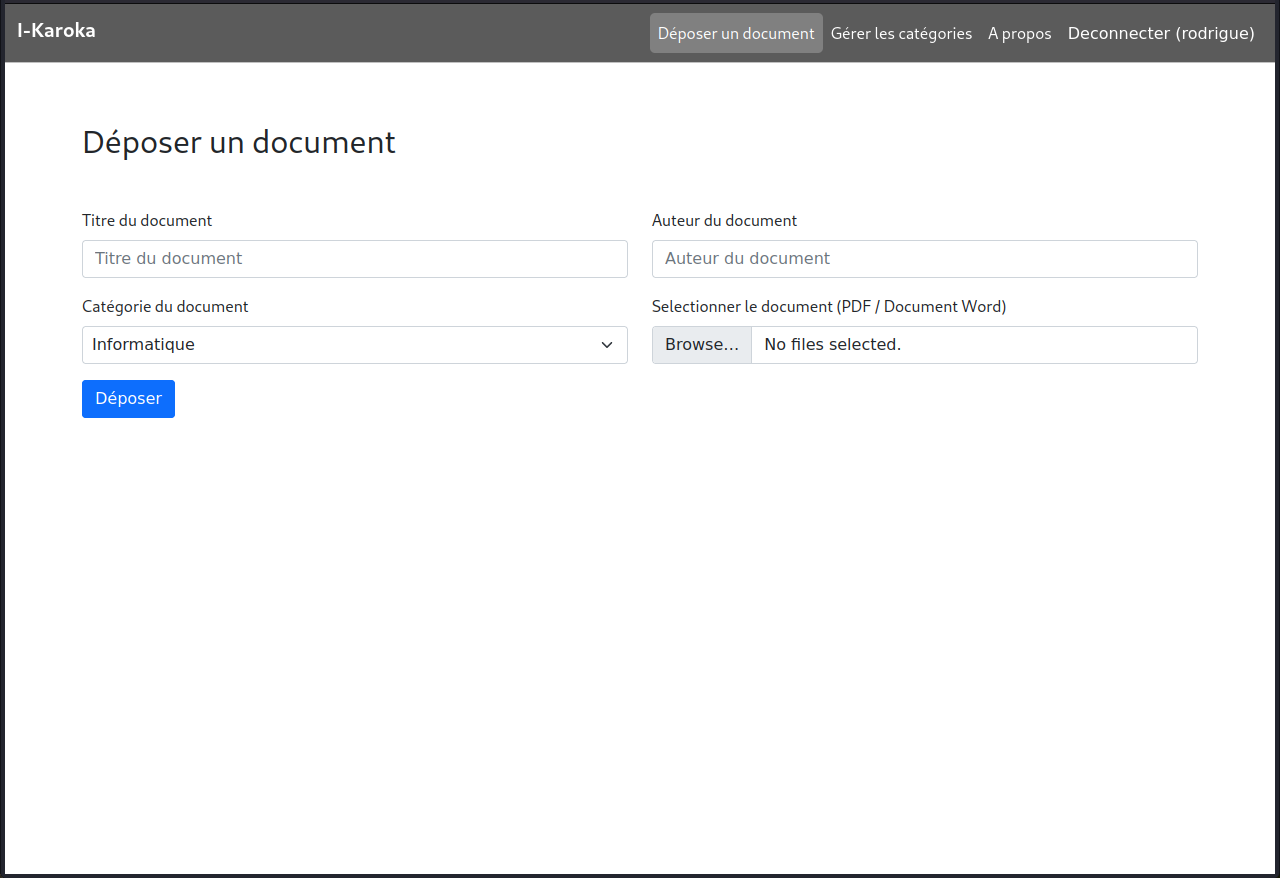
\includegraphics[width=15cm, angle=0]{Figures/Realisation/Demo/upload.png}}
    \end{center}
    \caption{Téléversement de document}\label{fig:doc-upload}
\end{figure}

\subsubsection{Recherche de document}
Supposons que la requête est: \og~moteur de recherche~\fg{} comme illustré dans la Figure~\ref{fig:search-index}. Le résultat sera la suivante avec les documents de test dans la base de donnés comme illustré dans la Figure~\ref{fig:search-results}.

\begin{figure}[htbp]
    \begin{center}
        \fbox{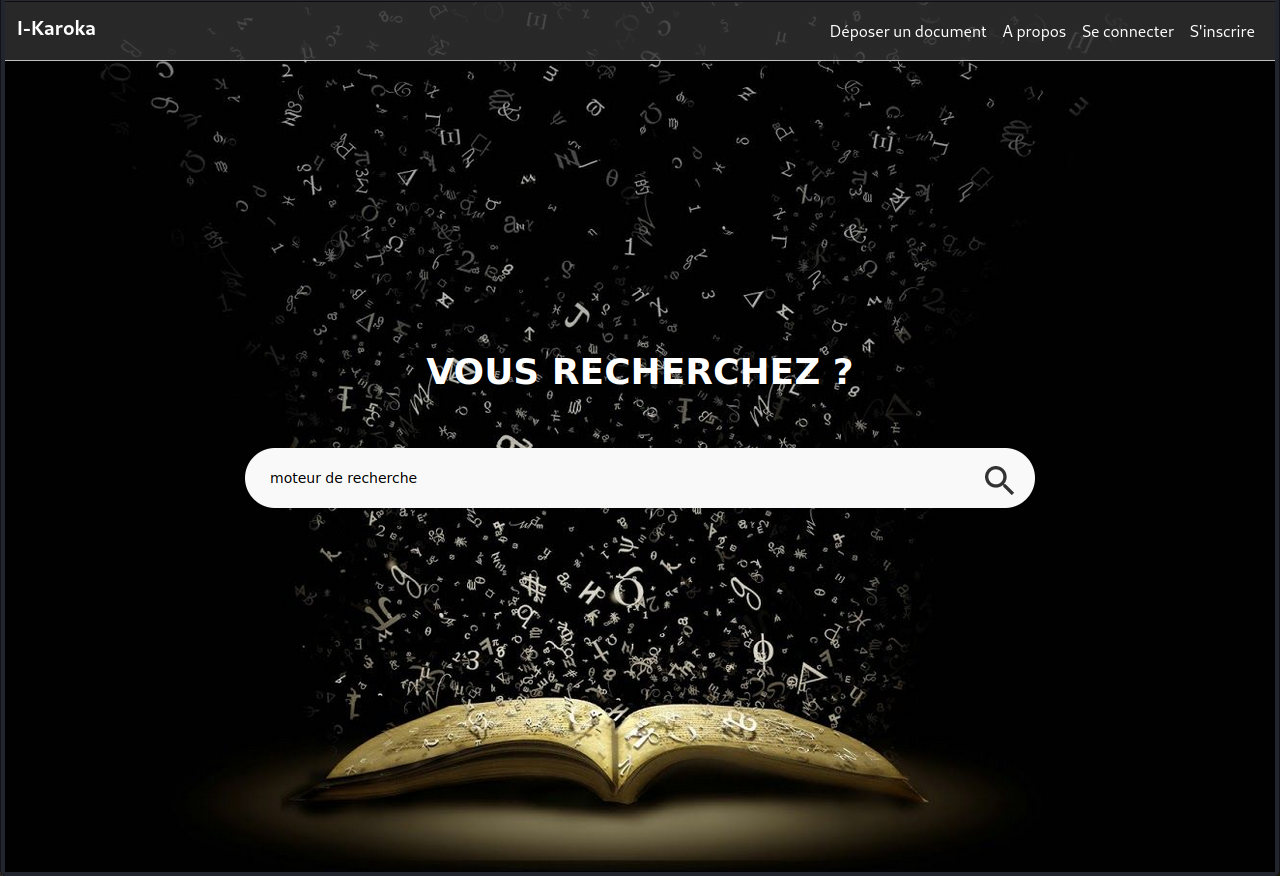
\includegraphics[width=15cm, angle=0]{Figures/Realisation/Demo/Index.png}}
    \end{center}
    \caption{Page d'accueil de recherche}\label{fig:search-index}
\end{figure}

\begin{figure}[htbp]
    \begin{center}
        \fbox{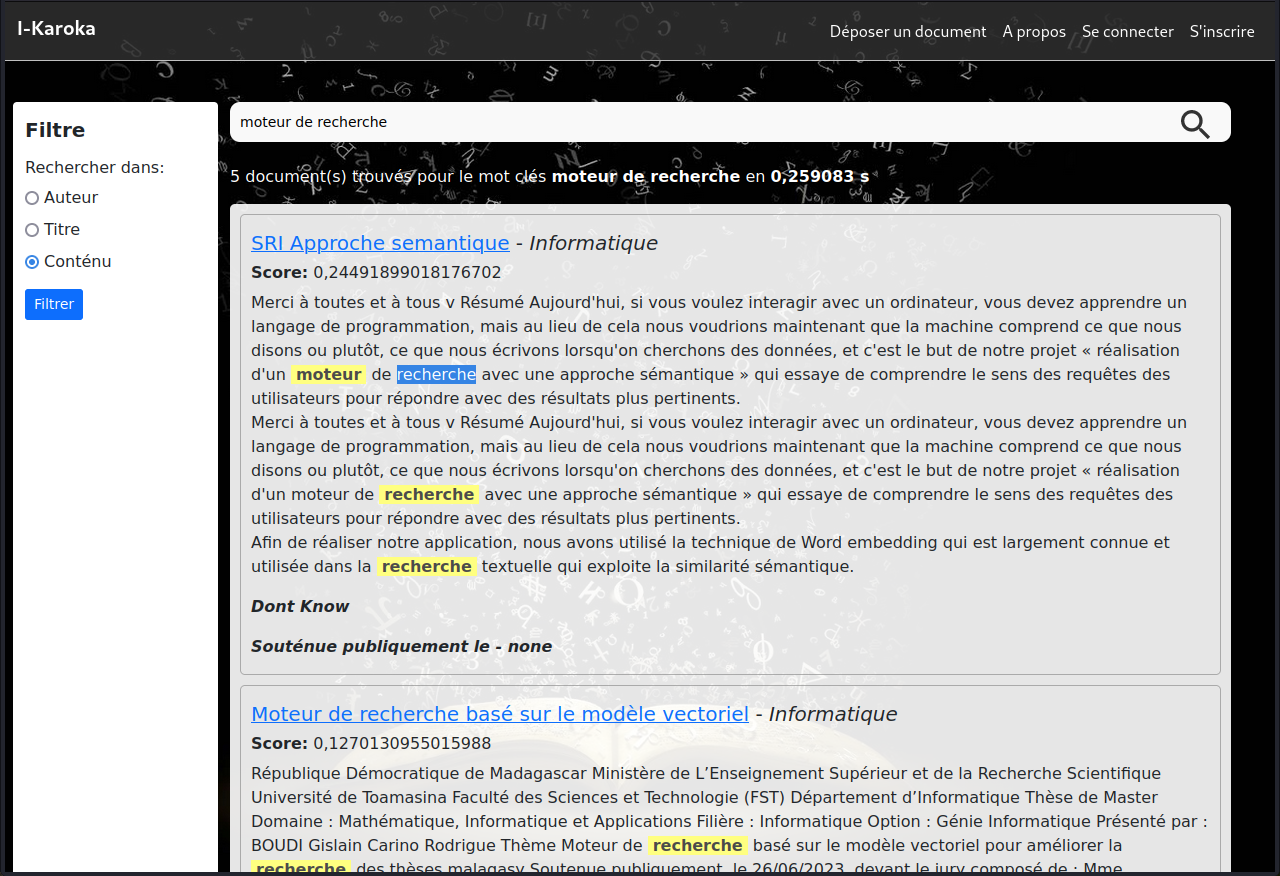
\includegraphics[width=15cm, angle=0]{Figures/Realisation/Demo/results.png}}
    \end{center}
    \caption{Résultat de recherche}\label{fig:search-results}
\end{figure}

\subsubsection{Visualisation et téléchargement}
La visualisation du document se fait par le clic du titre du document, et est illustré comme dans la Figure~\ref{fig:preview-download}
\begin{figure}[htbp]
    \begin{center}
        \fbox{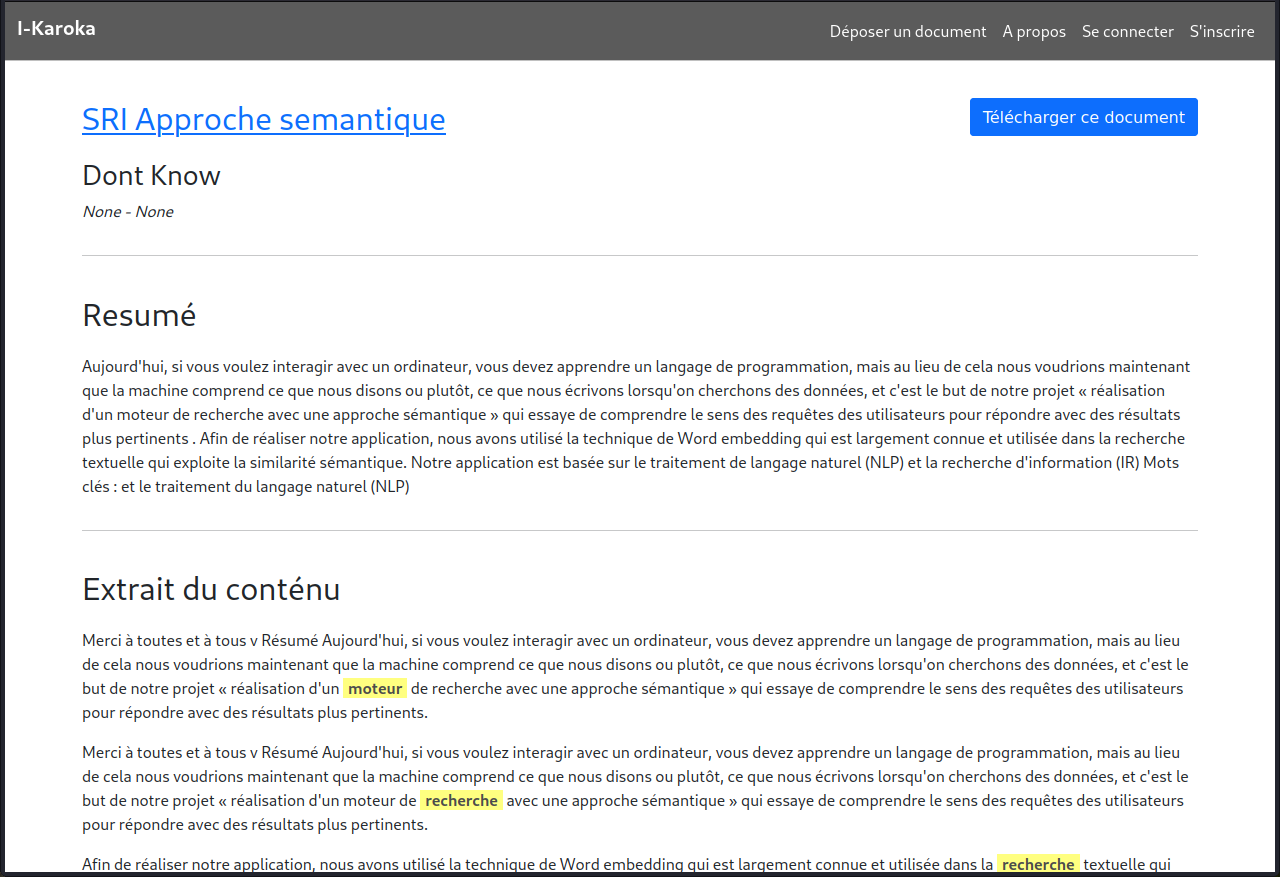
\includegraphics[width=15cm, angle=0]{Figures/Realisation/Demo/preview.png}}
    \end{center}
    \caption{Visualiser et télécharger un document}\label{fig:preview-download}
\end{figure}

% \section{Tests et validation du logiciel}
% \subsection{Stratégies de test utilisées pour évaluer la performance et la fonctionnalité du logiciel}
% \subsubsection{Tests unitaires}
% Description des tests unitaires réalisés pour vérifier le bon fonctionnement des composants individuels du logiciel.
% 
% \subsubsection{Tests d'intégration}
% Présentation des tests d'intégration effectués pour évaluer l'interopérabilité des différents modules du logiciel.
% 
% \subsubsection{Tests de validation}
% Explication des tests de validation effectués pour vérifier si le logiciel répond aux exigences spécifiées dans le cahier des charges.
% 
% \subsection{Résultats des tests et analyse critique des performances du logiciel}
% \subsubsection{Résultats des tests}
% Présentation des résultats détaillés des tests effectués, y compris les rapports de tests, les captures d'écran et les données de performance.
% 
% \subsubsection{Identification des problèmes}
% Discussion sur les éventuels problèmes ou erreurs identifiés au cours des tests, avec analyse critique des mesures prises pour corriger ces problèmes.

% \section{Implémentation du logiciel dans un contexte réel}
% \subsection{Processus d'implémentation}
% Pour implementer ce logiciel, il faut des thèses et mémoires malagasy (Master, Doctorat, Article, Révue scientifique) pour alimenter la bae de données. Puis catégoriser ces documents afin de faciliter l'indexation de ces documents. Une fois ces documents indexés, le système est fonctionnel.
% 
% \subsection{Évaluation de l'efficacité de l'implémentation}
% Analyse de l'efficacité de l'implémentation du logiciel en fonction des objectifs initiaux et des résultats observés dans le contexte réel.
% 
% \subsection{Rétroaction des utilisateurs}
% Présentation des retours d'expérience et des commentaires des utilisateurs finaux concernant l'utilisation et les performances du logiciel dans leur environnement réel.
% 
% \subsection{Réponses aux problèmes éventuels}
% Discussion sur la manière dont les problèmes éventuels rencontrés lors de l'implémentation ont été résolus, et sur les ajustements apportés pour améliorer l'expérience utilisateur et les performances du logiciel.

\section{Évaluation des performances et des résultats}
\subsection{Évaluation critique des performances du logiciel}
A rédiger
% Analyse approfondie des performances du logiciel en termes de fonctionnalité, de convivialité, de fiabilité et d'efficacité, en se référant aux critères établis au début du projet.

\subsection{Comparaison avec les objectifs initiaux}
A rédiger
% Comparaison des performances réelles du logiciel avec les objectifs initiaux définis lors de la conception, en mettant en évidence les écarts éventuels et les facteurs contributifs.

\subsection{Identification des forces et des faiblesses}
A rédiger
% Identification des points forts et des limitations du logiciel en fonction des retours d'expérience des utilisateurs et des évaluations techniques, en mettant l'accent sur les domaines nécessitant d'éventuelles améliorations ou ajustements.

\subsection{Implications et recommandations}
A rédiger
% Catégorisation des documents automatiques, extraction automatiques des titres, resumés, liste des bibbliographies, auteur, date de soutenance, encadreur ainsi que les membres de jury. Recupération des articles connexte. Création de bibliographie en connaissant ces informations.

% \section{Réflexions sur l'expérience de développement}
% \subsection{Analyse critique des leçons apprises}
% Analyse réfléchie des principaux enseignements tirés de l'expérience de développement du logiciel, en mettant l'accent sur les succès, les défis et les stratégies d'adaptation ou d'amélioration.
% 
% \subsection{Évaluation de l'efficacité des stratégies de développement}
% Évaluation de l'efficacité des différentes stratégies de développement utilisées tout au long du processus, en mettant en évidence les approches qui ont bien fonctionné et celles qui auraient pu être améliorées.
% 
% \subsection{Suggestions pour des améliorations futures}
% Proposition de suggestions concrètes pour améliorer les processus de développement, les stratégies de gestion de projet et les approches techniques pour de futurs projets similaires.
% 
% \subsection{Perspectives de recherche future}
% Discussion sur les pistes de recherche future potentielles basées sur les lacunes identifiées dans le cadre du projet actuel, en mettant l'accent sur les domaines qui méritent une exploration plus approfondie et des développements ultérieurs.